\chapter{System Architecture and Implementation}
\label{chap:archi}

Our main contribution in this paper is the creation of a brand action recognition algorithm. In this chapter, we will give a precise step-by-step description of our system.
\section{Hardware and Framework}
In this section, we will describe the hardware from which we obtained our data and the software elements that support our work.
\subsection{ROS Architecture}
Our algorithm is supposed to be applied on any domestic robot, and can become part of a larger robot control software. To make it portable and easy to plug to larger projects, we implemented it to be fully compatible with ROS.

ROS \cite{ROS} - for Robot Operating System - is not really a proper OS but rather a middleware that run on most Linux distributions whose primary task is to provide a robust support for large volumes of data that need to be processed in real time. It also makes it possible to paralellize a lot of programs even if some of the hardware does not have high performance CPU or GPU.

The basic principle of ROS is that it makes all the different programs work as nodes in a network. The most powerful computer of the network - in our case a desktop PC - hosts the ROS Core node and acts as a server: it is responsible for managing the exchange of data among all the other nodes. Each ROS node can do three basic actions: it can publish its output at a specified rate as ROS topics, which are then advertised by the Core node. It can also subscribe to topics published by other nodes, and can therefore use this data as real-time input for its own computations. Finally, it can propose ROS services to other nodes, which means that other nodes can exceptionally ask it for a specific data that is not published. 

The code for each node can be written in either C++ 11 or Python 2.7, and ROS can therefore also be useful to link the advantages of these two languages in one software. On this project, the computationally expensive code is written in C++ for its rapidity and the code for managing the data and transforming it is written in Python to make use of Numpy and other useful modules.

The ROS architecture is really robust for robotics since the computer that hosts the Core node can take care of the heavy computation tasks while the limited robot computer only has to send data to the network and get back the responses. Another big advantage of ROS is that it is extremely modulative: the hardware may change completely or you may add another or even ten robots to the system and all you have to do is to make sure that every node publishes and subscribes to the good topics. For all of these reasons, we chose ROS so that our software can be effective in many different environments with only little adaptation.

\subsection{Turtlebot}
The robot we used for our research is a Turtlebot2\footnote{https://www.turtlebot.com/turtlebot2/}. Turtlebot\textsuperscript{TM} is an easily programmable robot which consists in a Kobuki\footnote{http://kobuki.yujinrobot.com/about2/} base on top of which is mounted a Microsoft Kinect\textsuperscript{TM} sensor. 

The Kobuki\textsuperscript{TM} base contains four wheels including two motorised ones. A Kobuki\textsuperscript{TM} robot can rotate around itself and move forward and backward. The wheels provide odometry information - which will be useful for the mapping process - and the base also contains collision sensors.

The Kinect\textsuperscript{TM} sensor is the combination of a RGB camera and a IR sensor. The first version of the Kinect sensor also provides a Windows\textsuperscript{TM} development environment, but this is incompatible for ROS, which only runs on Linux. Because of that, we decided to use the second version instead: Kinect for XBox One\textsuperscript{TM}, since this version provides more accurate results\cite{kinect_comparison}. However, since there is no official driver release for this sensor, we instead use an open source one named libfreenect2\cite{libfreenect2}, which provides us both RGB and IR images, but no depth registration. Further explanation about the depth registration process and point cloud publication will be given later on this chapter.

We then use a program called kinect2 bridge\cite{iai_kinect2} to reconstruct the point cloud from the RGB and IR images. This is done by performing depth to color frame registration using extrinsic parameters of the Kinect cameras\footnote{\raggedright A description of the algorithm used can be found here: http://nicolas.burrus.name/index.php/Research/KinectCalibration}.
It then publishes 

\section{Unsupervised Pose Clustering}
In this section we describe how we obtain the pose estimation and create a cluster model from them.

\subsection{Dimensionality choice (move later ?)}
When we designed our workflow, we had to make a choice between estimating human action either from 2D or 3D human pose estimation. The tradeoff between the two techniques can be found in table \ref{tab:dimension_comparison}.

3D is a more natural environment for the robot since it already uses this coordinate system for mapping and navigation purpose. It also makes object segmentation easier since 3D point cloud data is sparse as opposed to images, we will detail that point in section \ref{section:object_rec}.

On the other hand, using 2D input is less computationally costly, and there are quick and reliable algorithm to perform body pose estimation like OpenPose, that we will describe in section \ref{section:openpose}. Another big advantage of 2D input is that image or video datasets are a lot easier to find than point cloud datasets. Because of all of these points, we decided to perform the clustering on 2D pose inputs.

\begin{table}[h]
    \centering
    \caption{Comparison of features between 2D and 3D environment}
    \label{tab:dimension_comparison}
    \begin{tabular}{|l|l|}
        \hline
        2D environment & 3D environment \\ \hline
        \textbf{+ Many image/video datasets available} & -- Datasets are rare \\
        + Easy to compute input & -- Computationally costly \\
        + Same algorithm for both human & -- Separate algorithms for the two tasks \\ detection and pose estimation & \\
        -- One dimension is not used & + Robot environment is in 3D \\
        -- Unsupervised object clustering: tricky & \textbf{+ Unsupervised object clustering} \\
        & \textbf{~~is easier (sparsity)}
        \\ \hline
    \end{tabular}
\end{table}

\subsection{2D Human Pose Estimation}
\label{section:openpose}
Human pose estimation is performed by using a trained deep learning model named OpenPose \cite{Openpose}. It takes image input and processes the body joint position for each individual present on the scene by computing part affinity field (PAF) fields. OpenPose performs quick enough for real-time applications: about 10 frames per second on our desktop PC. The outputs for each frame consists in the list of humans detected, where each human is represented as the list of his 18 body joints position as shown in fig \ref{fig:2D_joints_vis}. Each point consist in x and y coordinates of the joint on the image and a score confidence which represent the confidence the algorithm puts into this result. This confidence score will prove itself useful in the next steps of our algorithm.

\begin{figure}[ht]
    \centering
    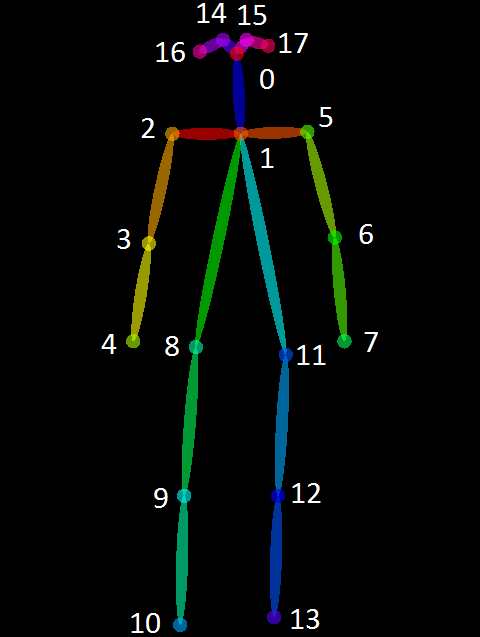
\includegraphics[width=80mm, keepaspectratio]{images/2D_body_joints_visualisation.png}
    \caption{2D human body joints visualisation}
    \label{fig:2D_joints_vis}
\end{figure}

\subsection{Unsupervised Clustering}
Most of unsupervised learning algorithms can be applied to pose estimation. In theory we could use as input anything, and we particularly considered using methods such as the classical and very simple K-means \cite{k_means} to more complete models such as self-organizing map \cite{self_organizing_map} or neural gas clustering \cite{neural_gas}.

However, we considered that an online algorithm would be better for our application, since it is more in accordance to a domestic robot environment: the robot should never stop learning to adapt itself constantly to the changes to the changes in its environment. Even with that constraint, a lot of different methods exist \cite{online_clustering_algo}, but in the end we decided to use the Self Organizing Incremental Network (SOINN) \cite{SOINN} to deal with our task. We chose this algorithm mostly because it is lightweight, operates in real-time and tackles efficiently the Stability-Plasticity Dilemma \cite{stability-plasticity_dilemma}. 

\begin{figure}[h]
    \centering
    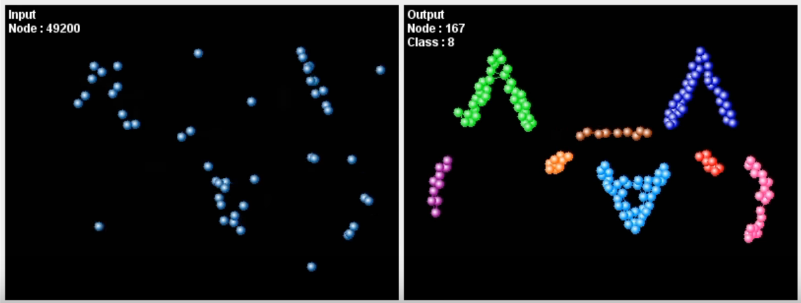
\includegraphics[width=150mm, keepaspectratio]{images/SOINN_cat.png}
    \caption{SOINN algorithm applied to noisy artificial data. For each step, random points from the original figure are selected along with pure noise points(left image). The algorithm assigns each new signal to a cluster, called node and reconfigure its architecture by recomputing its nodes values and the relationship between them (right image).}
    \label{fig:SOINN_cat}
\end{figure}

SOINN takes as input vectors of any dimensions - the only restriction is that these dimensions should remain consistent over time - and based on the distance between this new signal and the existing nodes either assigns the signal to an existing node or creates a new one. It then reconfigure its architecture and may decide to destroy nodes not used anymore or to fuse two nodes near to each others.
An example of clustering on artificial data is shown in figure \ref{fig:SOINN_cat}. 

\subsection{Pre-processing (experiments ?)}
Filters

For our application, we decided to discard the joints number 14 to 17 corresponding to the right/left eye and ears respectively. These joints did not affect the clustering result and were often either not detected at all or with a bad confidence score, which is problematic for the preprocessing part of our pose clustering algorithm.

\section{Spatial Context Acquisition}
description

\subsection{Navigation and Mapping}
SLAM

\subsection{3D Object Recognition}
\label{section:object_rec}
describe pcl workflow, RANSAC segmentation, euclidean cluster extraction, color-based segmentation

\subsection{3D Pose Estimation}
Openpose 3D

\section{3D Human-Object Interactions}

\subsection{Interaction Detection}
describe interaction detection method.

\subsection{Pose-Interaction Clustering}